\documentclass[10 pt,table]{article}  % Comment this line out
\usepackage{nips13submit_e,times}
\usepackage{hyperref}
\usepackage{url}
\usepackage{amsmath}
\usepackage{amssymb}
\usepackage{mathrsfs}

\usepackage{graphicx}

\usepackage{tabularx}
\usepackage{rotating}
\usepackage{url}
\usepackage{mathrsfs}
\usepackage{cite}
\usepackage{cancel}
\usepackage{multirow}

\usepackage{subfig}
% Figure
\newcommand{\figref}[1]{Fig.\ref{#1}}



%\documentstyle[nips13submit_09,times,art10]{article} % For LaTeX 2.09


\title{Improving matrix factorization}


\author{
Shrainik Jain (1323338)\\
\texttt{shrainik@cs.washington.edu} \\
\And
Arunkumar Byravan (1222561) \\
\texttt{barun@cs.washington.edu} \\
}

% The \author macro works with any number of authors. There are two commands
% used to separate the names and addresses of multiple authors: \And and \AND.
%
% Using \And between authors leaves it to \LaTeX{} to determine where to break
% the lines. Using \AND forces a linebreak at that point. So, if \LaTeX{}
% puts 3 of 4 authors names on the first line, and the last on the second
% line, try using \AND instead of \And before the third author name.

\newcommand{\fix}{\marginpar{FIX}}
\newcommand{\new}{\marginpar{NEW}}

\nipsfinalcopy % Uncomment for camera-ready version

\begin{document}


\maketitle

\begin{abstract}
Content Recommendation systems (eg. Netflix, Amazon) try to predict user responses for content to make a decision on recommending content to the user. One way to model this is to consider it as a matrix approximation problem. It has been shown that this problem can be solved using matrix factorization techniques by assuming that the matrix is of low rank. Lee et al \cite{lee2013local} relax this assumption and consider the matrix is locally low rank. They proceed to approximate this matrix as a smooth convex combination of low rank matrices each of which approximate local regions of the original matrix. We are interested in implementing this method and exploring ways to use context information to improve the predictions. We present our results for prediction accuracy using various types of context information and compare the results to the base algorithm.
\end{abstract}

\section{Introduction}
The Netflix Challenge, i.e., predicting a user's rating for a particular movie, has led to a significant amount of research in the field of Matrix factorization. This is because of the fact that the problem of predicting a user's rating of a movie, based on his ratings for other movies and ratings by other users for similar movies can be framed as solving a matrix approximation problem. If each user represents a row and each movie represents a column, then the problem is equivalent to finding the missing entries of this matrix. There are several approaches to solving this problem, most common among which are SVD \cite{paterek2007improving} (minimization of Frobenius norm) and Compressed sensing (minimization of nuclear norm). 

Most of the algorithms assume that the matrix is of a low rank. Lee et al \cite{lee2013local} relax this by assuming that the matrix is only locally low rank i.e., specific sub-regions of the matrix are of low rank. This assumption is strictly weaker than the global low rank approximation and the global approximation problem can now be decomposed into finding good low rank approximations for the sub-matrices. This results in a fast and easily parallelizable framework that works well on large sparse datasets. In this work, we implement the algorithm proposed in \cite{lee2013local} and test its performance on the MovieLens datasets. The algorithm in \cite{lee2013local} does not use contextual information for learning. By adding additional information on movie similarity, user age, gender etc we add priors to the learning algorithm to make better predictions. We are interested in exploring the effect of this biasing on the performance of the method in \cite{lee2013local}.

\section{Related Work}
There is a huge body of related work on solving the matrix approximation problem for recommendation systems. Common strategies can be broken to two broad categories \cite{koren2009matrix}, {\it content filtering} and {\it collaborative filtering}. Content filtering requires trained analysts to rate each content on various metrics and then match these metrics with the user choices. The obvious problem with this approach is that such metrics are often incredibly hard to collect or not available at all.

Collaborative filtering takes into account the user's past behaviour in terms of his preferences and does not require explicit profiling of content. Two primary methods in collaborative filtering are {\it neighbourhood methods} and {\it latent factor methods}. Neighbourhood methods look for other users with similar preferences and suggest the user with content that these other similar users like. Latent Factor methods represent a user's preference as a combination of several hidden factors. The final preference is dependent on the amount each factor matters to the user and how a movie fares on each of those factors.

In light of the netflix challenge, the problem was to build a recommendation system based on collaborative filtering using latent factor methods. This breaks down to the matrix approximation problem. After Billsus et al. \cite{billsus1998learning} initially proposed the use of SVD to solve collaborative filtering, there have been a number of similar approaches. Koren et al. \cite{koren2009matrix} talk about using SVD while including the effect of user bias and temporal dynamics in their model. Jaggi et al. \cite{jaggi2010simple} propose a novel tuning free approach to solve the problem by bounding the nuclear norm. The winners of the Netfilx prize \cite{bell2007modeling}\cite{sill2009feature} used an ensemble approach where the final prediction is a weighted combination of several methods like SVD, k-NN and Restricted Boltzmann Machines.

Given the scale of the data for the netflix challenge, the speed of prediction is also a very important factor and a number of works focus on finding distributed and parallizable solutions. Zhou et al. \cite{zhou2008large} use the Alternating-Least-Squares with Weighted-${\lambda}$-Regularization technique to solve a form of incomplete SVD and focus specifically on parallelizability. Mackey et al. \cite{mackey2011divide} provide a divide and conquer approach in which they break the problem into a number of smaller factorization problems and use SVD on each smaller problem. Lee et al. \cite{lee2013local} use a similar approach but with a key difference that they use distance based kernels to find subsets of dataset to work on and the subsets can overlap. In our work, we plan to use the idea from Lee et al. \cite{lee2013local} and incorporate contextual information to improve prediction accuracy.

Using contextual information in recommender systems has been proposed before. Adomavicius et al. \cite{adomavicius2005incorporating}\cite{adomavicius2011context} research this extensively and give the notion of context pre-filtering, post-filtering and modeling, which are different paradigms of incorporating context into predictions. We will be using similar approach to use context provided in the MovieLens1M and MovieLens10M to see if biasing the model produces better results.

\section{Theory}
In many content recommendation problems, there are observed ratings of different content by many users and given a new user, we have to choose specific content to recommend based on our model of the user's preference. We can think of this preference as being encoded in the user's ratings of other content and the ratings of similar users. We can construct a matrix $M$ of size $n_1 \times n_2$ ($n_1$ is the total \emph{number of users} and $n_2$ is the total \emph{number of different content}) with the observed ratings (set $A$). In practice, this matrix is usually sparse as we have ratings from only a few users on each content. The problem of predicting the user's preference for the remaining content can now be formulated as the problem of completing this matrix $M$ i.e. we want to find suitable values for the unknown entries of the matrix $M$ given the known set of ratings $A$. 

The predominant approaches to solving this problem construct an approximation $\hat{M}$ of the matrix $M$ by assuming that $M$ (and therefore $\hat{M}$) is of low rank. This means that we can approximate the matrix $M$ as:
\begin{align}
M \approx \hat{M} = UV^T \ ; \ U \in \mathbb{R}^{n_1 \times r}, V \in \mathbb{R}^{n_2 \times r}; r << min(n_1,n_2)
\end{align} 
It has been shown empirically that this assumption works well in practice \cite{paterek2007improving},\cite{koren2009matrix}. Two popular approaches to constructing this low rank approximation are:
\begin{itemize}
\item[$\mathcal{H}_1$] \emph{Incomplete SVD}:where we explicitly constrain the rank of the approximation to be $r$ and
\item[$\mathcal{H}_2$] \emph{Nuclear Norm minimization}:where minimizing the nuclear norm enforces low rankedness.
\end{itemize}
As an extension to these methods, Lee et al. \cite{lee2013local} propose a relaxation of the low rank assumption. Instead, they posit that the matrix $M$ is characterized by multiple low rank matrices each of which approximate $M$ in a local region. Given a specific point $(a,b)$ on the matrix, we have a mapping $\mathcal{T}(a,b)$ that approximates $M$ in the \textbf{local} region around the point $(a,b)$ with a low rank matrix. 

Key to this is an assumption of a metric structure over the rows and columns of $M$ (users and content respectively) with a specific distance metric $d((a,b),(c,d))$ measuring the similarity between users $a$, $c$ and items $b$, $d$. The metric $d$ defines the \textbf{local} region around any point and $\mathcal{T}(a,b)$ approximates $M$ in this local region. The authors make a key assumption that this mapping $\mathcal{T}$ is slowly varying (Holder continuous) which allows them to use a limited number of matrices $\mathcal{T}$ to approximate $M$ fully (otherwise, we need as many as $n_1n_2$ samples to estimate $\mathcal{T}$ accurately). Additionally, the authors define a smoothing kernel $K_h^{(a,b)}$ based on $d$ to smooth the contributions of other users and items while learning (a high value for a specific (user,movie) pair leads the algorithm to try to estimate it better). With this general idea in mind, we can look at local versions of the two algorithms mentioned above as they try to estimate $\mathcal{T}(a,b)$ as a low rank matrix $\hat{\mathcal{T}}(a,b)$ for a point $(a,b)$:
\begin{itemize}
\item[$\mathcal{H'}_1$] \emph{Incomplete SVD}: 
\vspace{-2mm} \begin{align}
 \hat{\mathcal{T}}(a,b) &= \arg \min_{\hat{\mathcal{T}}} \sum_{(a',b') \in A} K_h^{(a,b)}(a',b') \left([UV^T]_{(a',b')} - M_{(a',b')}\right)^2 \\
&s.t. \ \ \ rank(\hat{\mathcal{T}}(a,b)) = rank(UV^T) = r
\end{align} 
\item[$\mathcal{H'}_2$] \emph{Nuclear Norm minimization}:
\vspace{-2mm} \begin{align}
&\hat{\mathcal{T}}(a,b) = \arg \min_{\hat{\mathcal{T}}} \left\| \hat{\mathcal{T}}(a,b) \right\|_* \\
&s.t. \ \ \ \sum_{(a',b') \in A} K_h^{(a,b)}(a',b') \left([UV^T]_{(a',b')} - M_{(a',b')}\right)^2 < \epsilon
\end{align}
\end{itemize}
This gives us a low rank approximate of $M$ in a local region around $(a,b)$. Repeating this process for a few different $(a,b) \in Q$ values gives us low rank approximates in different areas of $M$. Given a new test entry $(c,d)$ we can predict the mapping around the point as:
\vspace{-2mm}\begin{align}
\hat{\hat{\mathcal{T}}}(c,d) = \sum_{(a,b) \in Q} \frac{K_h^{(a,b)}(c,d) \hat{\mathcal{T}}(a,b)}{\sum_{(a',b') \in Q} K_h^{(a',b')}(c,d)}
\end{align}
This leads to a simple algorithm for Local LOw Rank Matrix Approximation (LLORMA) where we choose a random set of points $Q$ and learn the low rank mappings $\hat{\mathcal{T}}$ around them using the local version of incomplete SVD ($\mathcal{H'}_1$) with additional regularization on the matrices $U$ and $V$. As the points $Q$ are chosen randomly, learning at each point can be done in parallel. 

\section{Adding Contextual information}
Incorporating context information into predictions has been researched separately \cite{adomavicius2005incorporating}\cite{adomavicius2011context}, but most matrix factorization techniques do not make use of context. Increasing the rank $r$ of the decomposition for incomplete SVD should give an effect similar to the addition of context as the number of latent features increase with $r$. But a larger rank results in increasing computational complexity and this becomes difficult for large datasets. Using context information, we should be able achieve similar results at lower rank values.

In LLORMA, similarity between the users and movies is used to compute a local region around a given anchor point to which the low rank decomposition is applied. At test time, this similarity is used to guide the prediction given a new user and movie pair. Therefore, the measure of similarity is critical to the performance of the algorithm (assuming that using similarity is a good idea in general) and we posit that biasing this measure with additional contextual information may give us better prediction performance. We look at combining this information with the original similarity measure to gauge its effect on prediction performance. 

We looked at two methods for adding contextual information into LLORMA:
\begin{itemize}
\item[\textbf{\emph{Method 1}}]: Biasing the kernel ($K_h$) using contextual information in addition to cosine similarity before training and using this biased measure for training and testing
\item[\textbf{\emph{Method 2}}]: Biasing the kernel after training and using it only for the testing phase (the original similarity measure from \cite{lee2013local} is used for training)
\end{itemize}
\figref{fig:simMethods} shows a pictorial depiction of the methods. The Movielens-1M dataset has information on user age, gender, location and movie genre while the Movielens-10M dataset has information on movie genres. We do not test against the Netflix dataset as we could not find good contextual information (except rating date) for it.

\begin{figure}[h!]
\centering
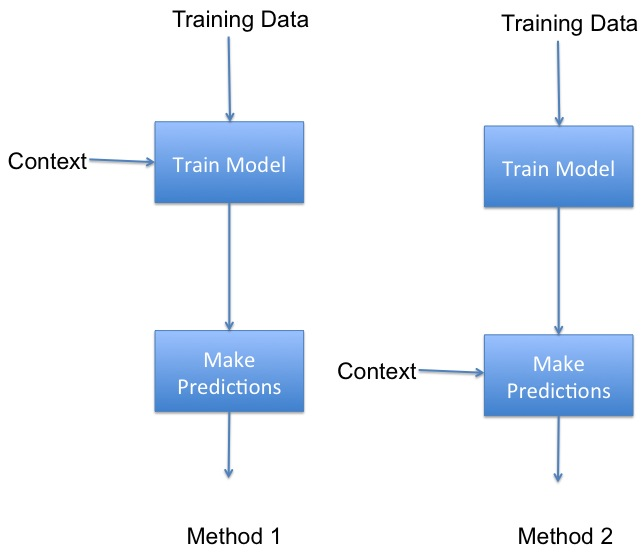
\includegraphics[width=0.4\columnwidth]{simMethods}
\caption{\small Methods of incorporating contextual information into LLORMA}
\label{fig:simMethods} \vspace{-1mm}
\end{figure} 

\section{Experiments}
In the original paper \cite{lee2013local}, the authors tested the algorithm on the MovieLens and Netflix datasets. The distance metric $d$ was computed as the angle between the singular vectors (rows \& columns of $U$ and $V$ respectively) and $K_h$ was chosen to be an epanechnikov kernel that decomposes over users and items. 
 
\subsection{Baseline}
We implemented the LLORMA algorithm in MATLAB with the same settings as in the original paper and tested it on the MovieLens1M and MovieLens10M datasets. As expected, we were able to match the RMSE ranges shown in the original paper (the values are not exact due to randomization). Table \ref{table:contextRMSE1M} and \ref{table:contextRMSE10M} shows the RMSE values for LLORMA on the MovieLens datasets with 50 anchor points and varying rank. These results serve as the baseline for further comparison of the performance of LLORMA with the addition of contextual information.

\subsection{Age}
We first use age to bias the user similarity. For a given user, the similarity to other users based on age is computed in the following manner:
\begin{align}
s_{age} = 6 / (|Age_{user1} - Age_{user2}|) \,\,\, for,\,\,\, Age_{user1} \neq Age_{user2} \\
s_{age} = 1 \,\,\, for,\,\,\, Age_{user1} = Age_{user2}
\end{align} \label{eq:simAge}
and this is added to the kernel using:
\begin{align}
K_h = K_h * s_{age}
\end{align} \label{eq:kernelAge}
The idea behind using the similarity measure as defined above is that MovieLen1M dataset has Age given as age groups, in groups like 18-25, 25-32, so on, and age value of 18 means that the user's age is the in group 18-25. The above measure considers same age group similarity as 1, adjacent age groups similarity as 0.85 and so on. We also tried similarity functions using exponential of age differences, which gives similar results. The resulting RMSE values with the addition of age information on the MovieLens 1M dataset for different rank $r$ is shown in the second row of table \ref{table:contextRMSE1M}. Training using the updated kernel (method 1) seems to perform worse than training normally and using the kernel at test time (method 2), but both of them do worse than the baseline meaning that adding age similarity actually worsens the performance of LLORMA.

\begin{table}
\begin{center}
\begin{tabular}{cc|c|c|c|c|}
\cline{3-6}
& & Rank-3 & Rank-5 & Rank-7 & Rank-10 \\ \cline{1-6}
\multicolumn{2}{|c|}{Baseline} & 0.8834 & 0.8584 & 0.8520 & 0.8499 \\ \cline{1-6}
\multicolumn{1}{ |c| }{\multirow{2}{*}{Age} } &
\multicolumn{1}{ |c| }{Method-1} & 0.8871 & 0.8585 & 0.8540 & 0.8510     \\ \cline{2-6}
\multicolumn{1}{ |c  }{}                        &
\multicolumn{1}{ |c| }{Method-2} & 0.8840 & 0.8586 & 0.8531 & 0.8508     \\ \cline{1-6}
\multicolumn{1}{ |c| }{\multirow{2}{*}{Gender} } &
\multicolumn{1}{ |c| }{Method-1} & 0.8840 & 0.8594 & 0.8538 & 0.8502     \\ \cline{2-6}
\multicolumn{1}{ |c  }{}                        &
\multicolumn{1}{ |c| }{Method-2} & 0.8841 & 0.8593 & 0.8534 & 0.8499     \\ \cline{1-6}
\multicolumn{1}{ |c| }{\multirow{2}{*}{Movie Genre} } &
\multicolumn{1}{ |c| }{Method-1} & 0.8797 & 0.8597 & 0.8526 & 0.8501     \\ \cline{2-6}
\multicolumn{1}{ |c  }{}                        &
\multicolumn{1}{ |c| }{Method-2} & 0.8793 & 0.8583 & 0.8533 & 0.8499     \\ \cline{1-6}
\multicolumn{1}{ |c| }{\multirow{2}{*}{Combined} } &
\multicolumn{1}{ |c| }{Method-1} & 0.8847 & 0.8623 & 0.8552 & 0.8500     \\ \cline{2-6}
\multicolumn{1}{ |c  }{}                        &
\multicolumn{1}{ |c| }{Method-2} & 0.8835 & 0.8594 & 0.8537 & 0.8500     \\ \cline{1-6}
\end{tabular}
	\caption{\small{RMSE values for LLORMA with context added on the MovieLens-1M dataset. Results averaged over 20 tests.}}
	\label{table:contextRMSE1M}
	\end{center}
\end{table}

\subsection{Gender}
Next we try using gender to bias the user similarity. For a given user, the similarity to other users based on gender is computed in the following manner:
\begin{align}
s_{gender} = c \,\,\, for,\,\,\, Gender_{user1} \neq Gender_{user2} \\
s_{gender} = 1 \,\,\, for,\,\,\, Gender_{user1} = Gender_{user2} \\
where \,\,\, c \, \epsilon \, [0, 1)
\end{align} \label{eq:simGender}
and this is added to the kernel using:
\begin{align}
K_h = K_h *s_{gender}
\end{align} \label{eq:kernelGender}
We ran the experiments with $c$ in [0.1, 0.2, 0.3, 0.4, 0.5, 0.6, 0.8, 0.9]. The prediction acurracy (in terms of RMSE) worsens with decreasing $c$. This is expected as reducing $c$ increases the bias of the model.
The results for $c = 0.9$ are shown in third row of table \ref{table:contextRMSE1M}.

\subsection{Movie Genre}
Movie Genre information is available for both the MovieLens1M and MovieLens10M datasets. Each movie entry has the names of the different classes it falls in (comedy, horror etc). To compute similarity based on movie genre, we created a binary vector ($m^{genre}$) for each movie where a 1 meant that the movie belonged to that genre and vice versa. The length of this vector is equal to the total number of genres in the dataset. We then combined it with the corresponding row in the $V$ matrice as in section 3 using a simple horizontal merge to row vectors $m^{combined}$. The rationale behind this is that a rank r factorization yields a matrix $V$ with $r$ latent factors, we do not want to loose the information of these latent features. We then use the cosine similarity metric between these combined vectors to compute the similarity between different movies:
\begin{align}
s_{genre} = 1 - \frac{2}{\pi}\arccos\left(\frac{m_j^{combined} \cdot m_k^{combined}}{\left\|m_j^{combined}\right\| \left\|m_k^{combined}\right\|}\right)
\end{align}
and add the result to the kernel as:
\begin{align}
K_h = K_h *s_{genre}
\end{align}
Results for using genre similarity for the MovieLens1M and MovieLens10M datasets are given in tables \ref{table:contextRMSE1M} and \ref{table:contextRMSE10M} respectively. \figref{fig:genreRMSE1M} and \figref{fig:genreRMSE10M} depict these results pictorially. The prediction performance for both the methods is better than that of the baseline which tells us that the additional similarity information from movie genre is indeed useful for prediction. We also tried experimenting with similarity measure dependent on only the cosine similarity of $m^{genre}$ binary vectors and not the $combined$ vector for the calculation of $s_{genre}$, but that biases the model too much and the results are worse than baseline algorithm.

\begin{table}
\begin{center}
\begin{tabular}{cc|c|c|c|c|}
\cline{3-6}
& & Rank-3 & Rank-5 & Rank-7 & Rank-10 \\ \cline{1-6}
\multicolumn{2}{|c|}{Baseline} & 0.8260 & 0.8138 & 0.8029 & 0.7978 \\ \cline{1-6}
\multicolumn{1}{ |c| }{\multirow{2}{*}{Movie Genre} } &
\multicolumn{1}{ |c| }{Method-1} & 0.8221 & 0.8132 & 0.8021 & 0.7943     \\ \cline{2-6}
\multicolumn{1}{ |c  }{}                        &
\multicolumn{1}{ |c| }{Method-2} & 0.8255 & 0.8122 & 0.8078 & 0.7978     \\ \cline{1-6}
\end{tabular}
	\caption{\small{RMSE values for LLORMA with added movie genre similarity on the MovieLens-10M dataset. Results averaged over 20 tests}}
	\label{table:contextRMSE10M}
	\end{center}
\end{table} 

\begin{figure*}[t!]
\centering
 \subfloat[MovieLens1M]{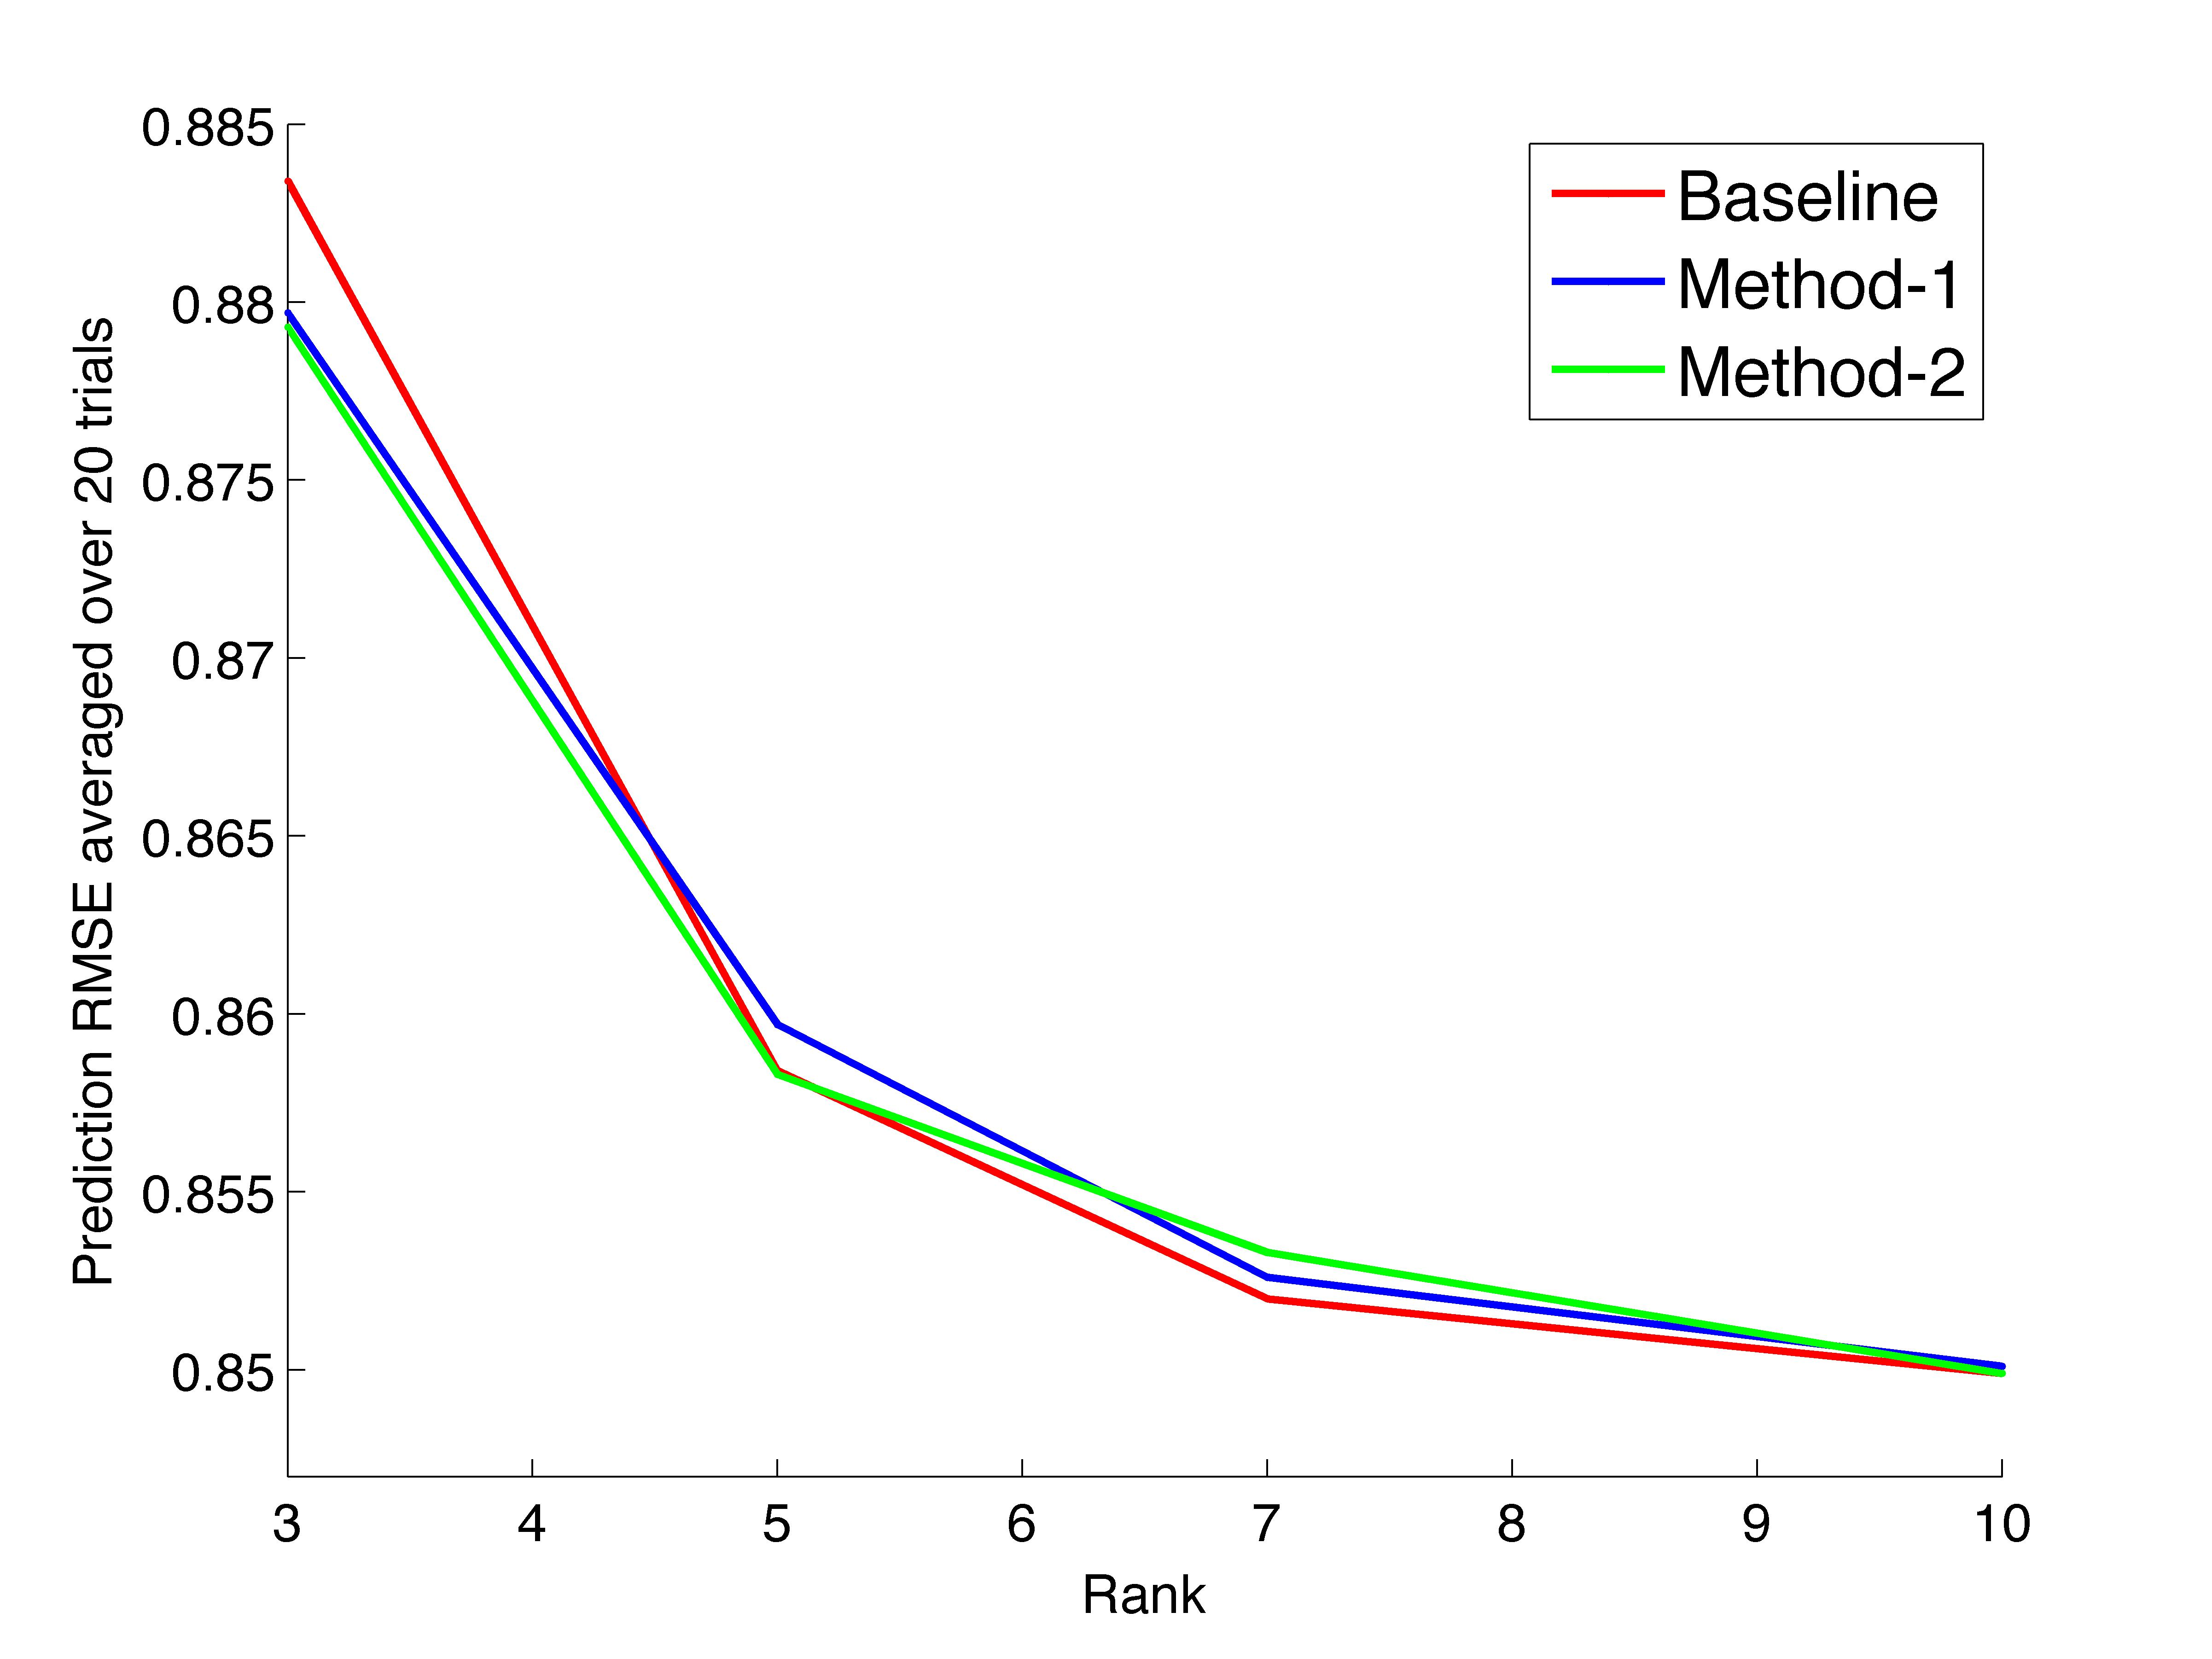
\includegraphics[width=0.53\columnwidth]{MovieLens1MGenre}\qquad\quad
\label{fig:genreRMSE1M}}
 \subfloat[MovieLens10M]{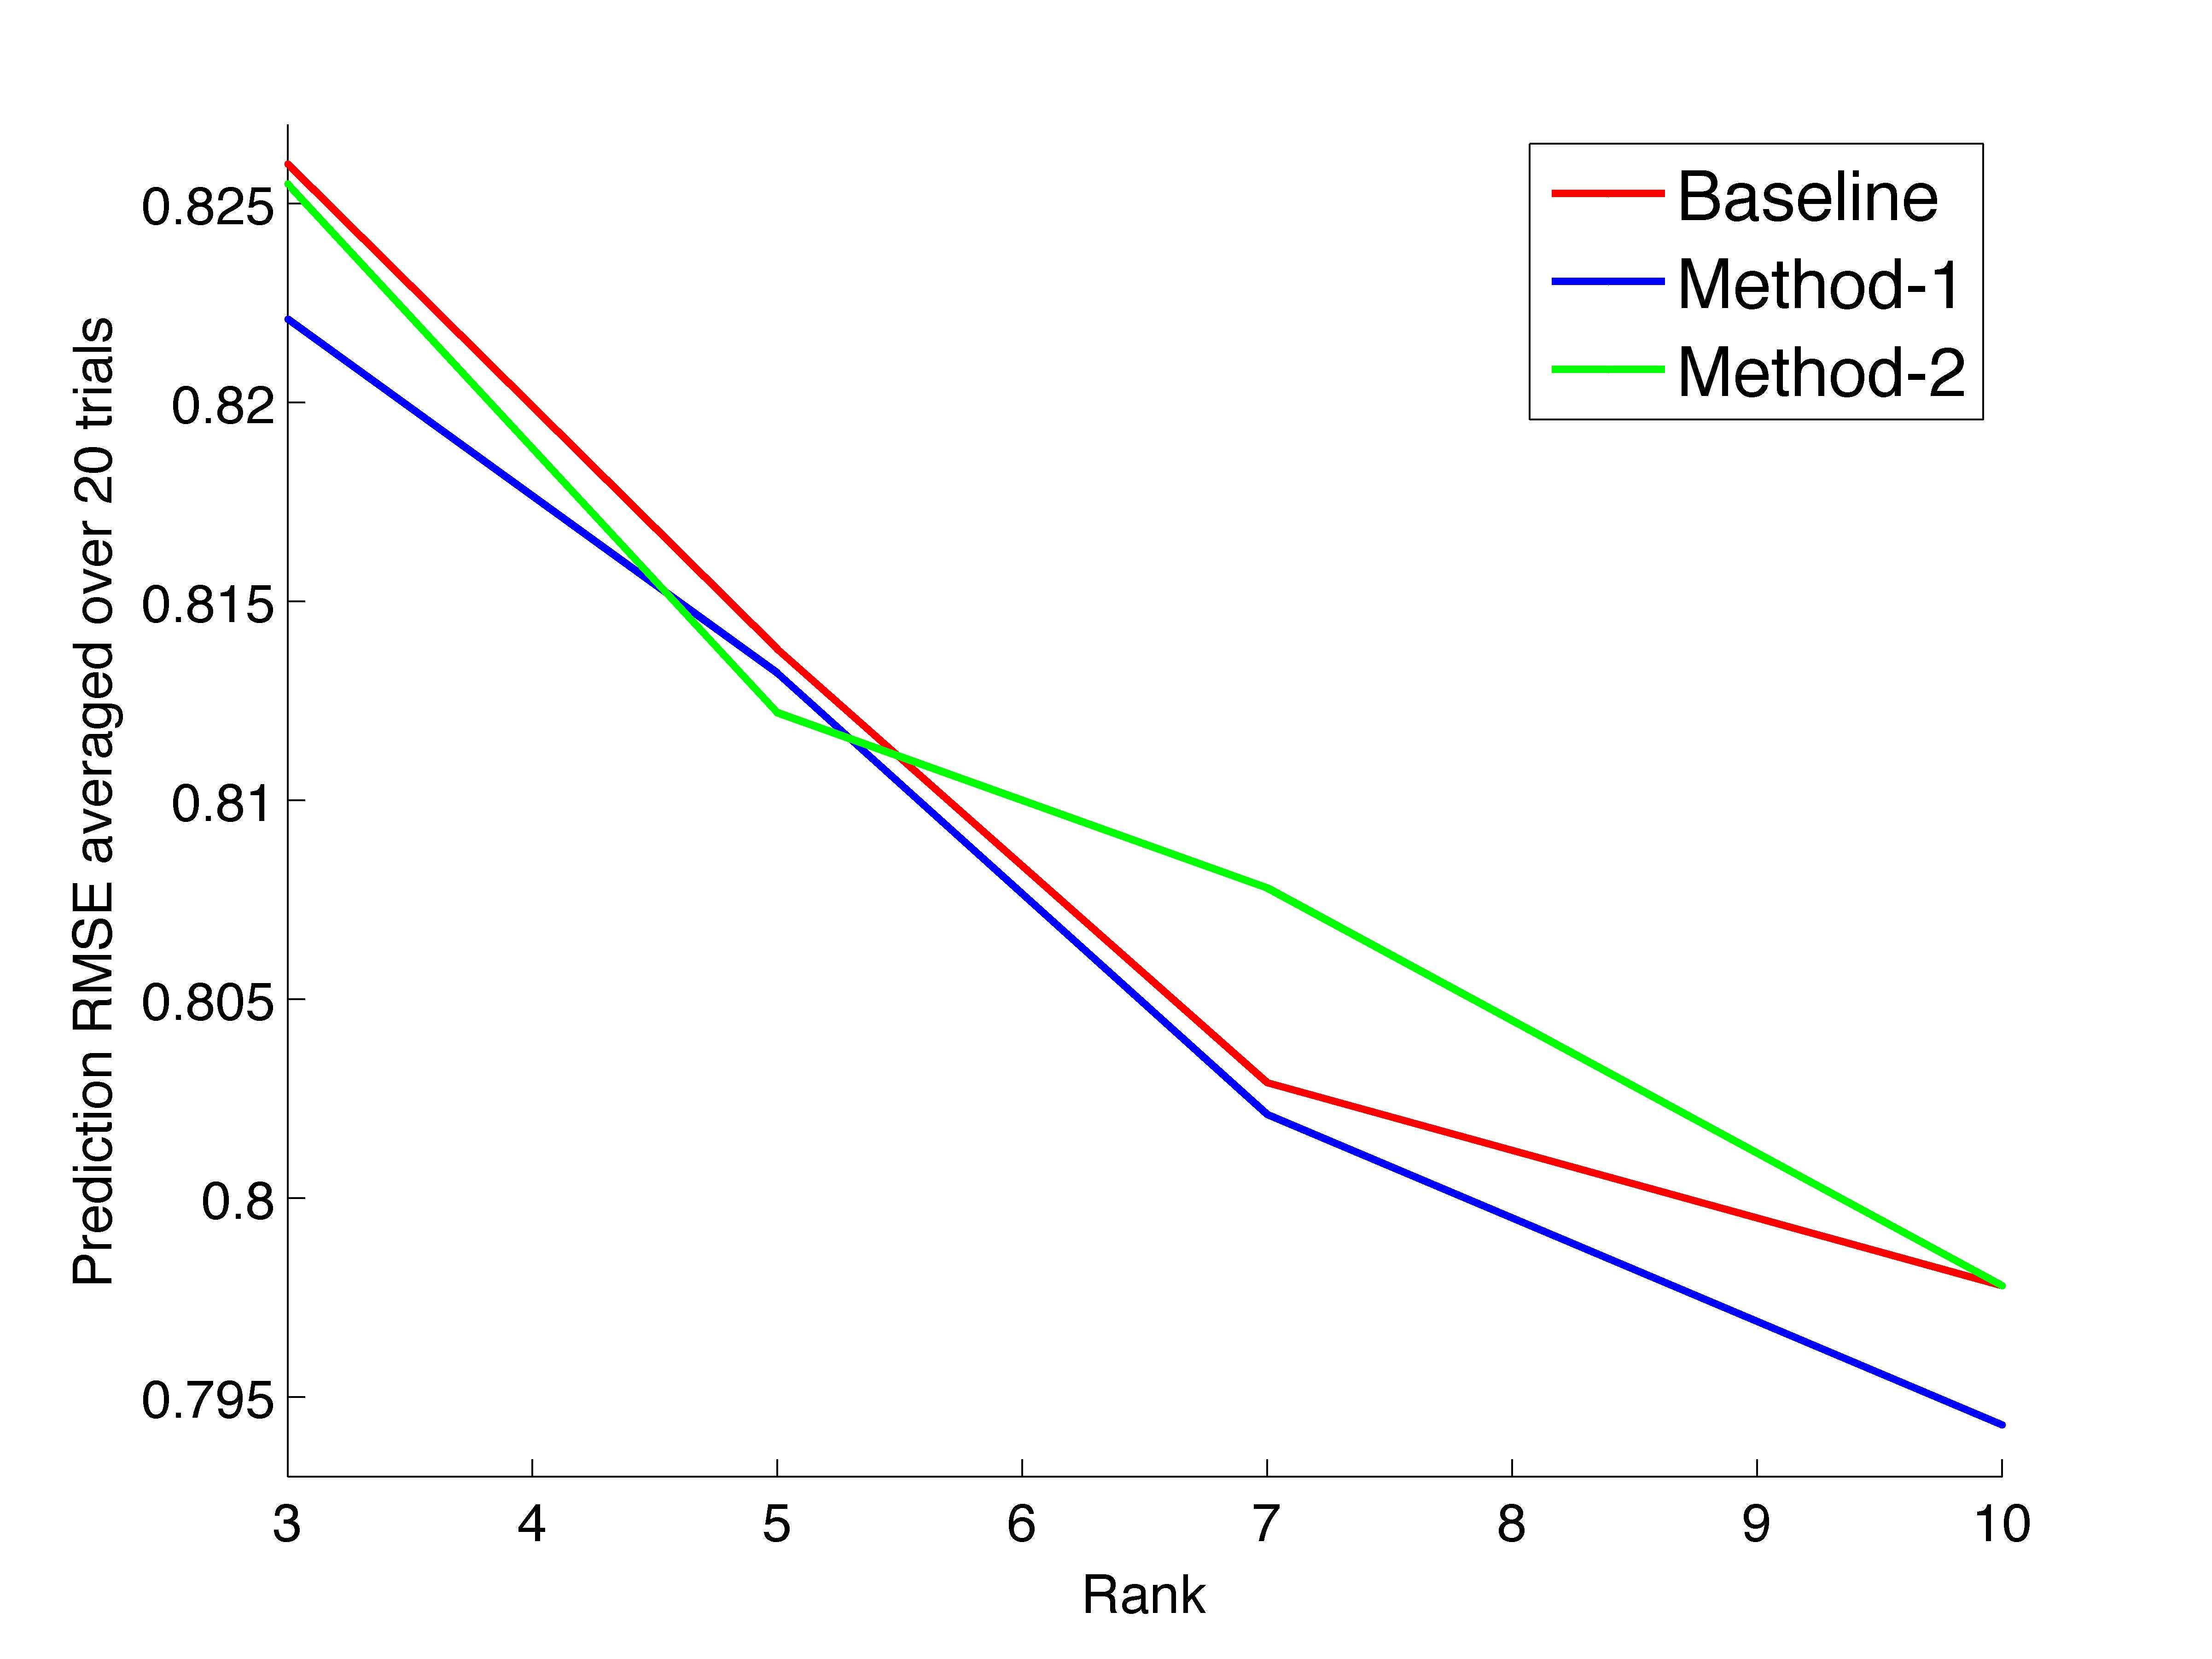
\includegraphics[width=0.53\columnwidth]{MovieLens10MGenre}\qquad\quad
\label{fig:genreRMSE10M}}
\caption{\small RMSE values for addition of movie genre information to LLORMA on MovieLens1M and MovieLens10M datasets averaged over 20 tests.}
\label{fig:TCH_2DTraj1}\vspace{-4mm}
\end{figure*}


\subsection{Combined}
Finally we tried combining the all these context measures to analyze the corresponding results. This was a simple update to the kernel $K_h$ as follows:
\begin{align}
K_h = K_h *s_{age}*s_{gender}*s_{genre}
\end{align}
The results are shown in last row of table \ref{table:contextRMSE1M}.
\subsection{Interpretation of results}
For locally low rank matrix factorization, use of user context like age, gender doesn't help in predictions, infact the base algorithm always beats it. This is expected as the ratings by users are not  heavily dependendent on age or gender, but they would depend a lot on the genre of the movie. Our experiments suggest that for the genre context, both methods of using context work better than the base algorithm until a certain rank. Context information as used, doesnt help much high ranks, a possible reason for this is that at higher ranks, the number of latent factors considered by the base algorithm automatically take into account the genres as hidden features of a movie. But, for very large datasets (Netflix, MovieLens 10M), when it might be costlier to use higher rank computations, we can use context to make computations faster at a small cost to RMSE. Finally, the use of all the context filters at the same time gives the worst results, this is because the model then becomes heavily biased towards specific users and movies.

\section{Limitations and Future Work}
We show that it is possbile to improve predictions using context, but the improvement is not very significant. We believe that we used very simple methods to add contextual information and better kernels and more complicated measures might give better results. Also, not all datasets provide context information (eg netflix), so using context is either not possible or requires merging data sets from multiple sources. Finally, for smaller datasets, LLORMA works better without context information as we can increase r to much higher values without incurring the computational costs. One major area for future work is in testing the performance on different datasets with different contexts and better similarity measures. We are also interested in an efficient parallel implementation of this algorithm. Finally, we are looking at developing an online version of this algorithm.

\section{Conclusion}
We have shown that the addition of contextual information improves prediction accuracy \textbf{\emph{(albeit slightly)}} for the local low rank matrix factorization technique. Among the different contextual information we used, movie genre seems to be the most informative. These results support the claim that contextual information can be useful for content recommendation systems and combining this with matrix factorization techniques can give good performance upto a certain rank. Since higher rank factorizations can be computationally expensive, we show that we can get similar performance at a lower rank if we use context information.

\subsubsection*{Acknowledgments}
Most of the work in this report is derived from the Local Low-Rank Matrix approximation paper \cite{lee2013local} by Lee et al.

\bibliographystyle{IEEEtran}
\bibliography{references}

\end{document}
